\documentclass[a4paper,12pt]{article}
\usepackage[utf8]{inputenc}
\usepackage[T1]{fontenc}
\usepackage[french]{babel}
\usepackage{graphicx}
\usepackage{amsmath}
\usepackage{a4wide}
\usepackage{subfig}
\usepackage{wrapfig}
\usepackage{url}
\usepackage{latexsym} % \Join
\usepackage[pdftex]{hyperref}
\hypersetup{
  colorlinks,
  citecolor=black,
  filecolor=black,
  linkcolor=black,
  urlcolor=black
}
\usepackage[top=2.5cm, bottom=2.5cm, left=2cm, right=2cm]{geometry}
%\renewcommand{\baselinestretch}{1.05}

\usepackage{listings}

\title{INFO-H-301: Lemmings}

\author{Quentin \textsc{Stiévenart}}
\date{\today}

\newcommand{\HRule}{\rule{\linewidth}{0.5mm}}

\begin{document}

\maketitle

\HRule

\section{Fonctionnalités}

Le programme réalisé consiste en un clone du jeu \emph{Lemmings} et
tire ses données graphiques de deux jeux libres:
\emph{Pingus}\footnote{\url{http://pingus.seul.org}} et
\emph{Teeworlds}\footnote{\url{http://teeworlds.com}}.

Au lancement du jeu, un menu est présenté à l'utilisateur (voir figure
\ref{fig:Menu}) et permet de:
\begin{list}{-}{}
  \item lancer le jeu~;
  \item choisir la carte sur laquelle jouer~;
  \item voir les meilleurs scores pour une carte~;
  \item changer les options graphiques (résolution, plein écran) et
    appliquer ces changements~;
  \item quitter.
\end{list}


\begin{figure}[ht!]
  \centerline{
  \subfloat[Le menu du jeu]{\label{fig:Menu}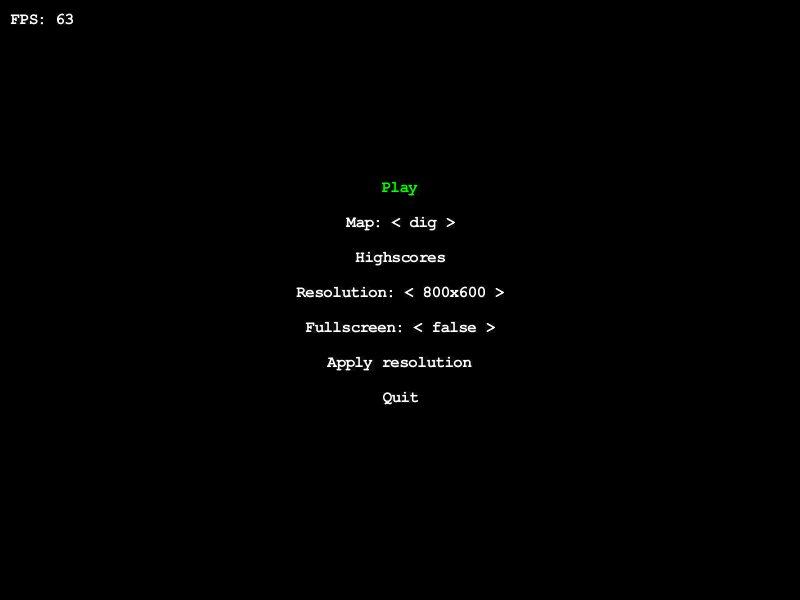
\includegraphics[width=0.55\textwidth]{menu.png}}
  ~~~~~~
  \subfloat[Le jeu]{\label{fig:Jeu}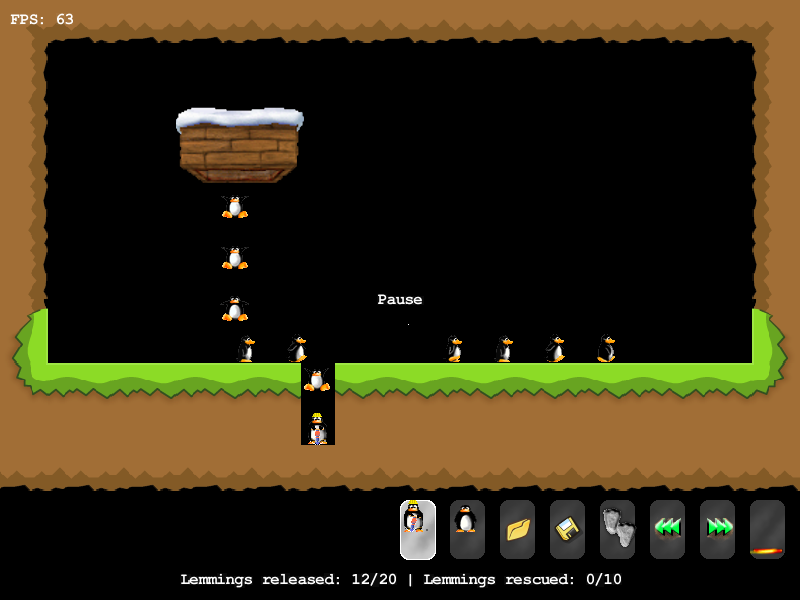
\includegraphics[width=0.55\textwidth]{jeu.png}}}
  \caption{Captures d'écran}
\end{figure}

Les meilleurs scores ainsi que les paramètres graphiques sont sauvegardés
dans une base de donnée, et sont donc conservés entre deux lancements du
jeu.\\

Lorsque le jeu est lancé, les lemmings sortent un par un depuis
l'entrée. Le but du jeu est de les conduire jusqu'à la sortie (les
cartes contiennent exactement une entrée et une sortie). Pour arriver
à cette fin, l'utilisateur peut donner différents \emph{comportements}
aux lemmings (creuser, exploser, \dots).\\

Le joueur a aussi la possibilité de mettre la partie en pause,
d'augmenter ou diminuer la vitesse du jeu, d'abandonner une partie (en
faisant exploser tous les lemmings) et de sauver ou charger une
partie.\\

À la fin du jeu (lorsque tous les lemmings sont soit sortis, soit
morts), l'utilisateur est invité à entrer son nom pour sauver son
score dans la base de donnée.\\

Le jeu a été réalisé avec les bibliothèques graphiques
\emph{Slick}\footnote{\url{http://slick.cokeandcode.com/}} et
\emph{LWJGL}\footnote{\url{http://www.lwjgl.org/}} afin de pouvoir
manipuler directement les textures OpenGL des images pour pouvoir les
modifier, ce qui est nécessaire pour que les lemmings puissent creuser
dans la carte.

\section{Diagramme de classes et architecture orientée objet}
Le programme est réalisé selon le patron de conception \emph{modèle
  vue contrôleur}.

\subsection{Modèle}
Le modèle est implémenté dans le package \texttt{model}. Il contient
les classes \texttt{Map} et \texttt{Character} qui héritent de la
classe \texttt{Entity} (une entité est un objet avec une position et
une taille).

\begin{figure}[ht!]
  \centerline{
  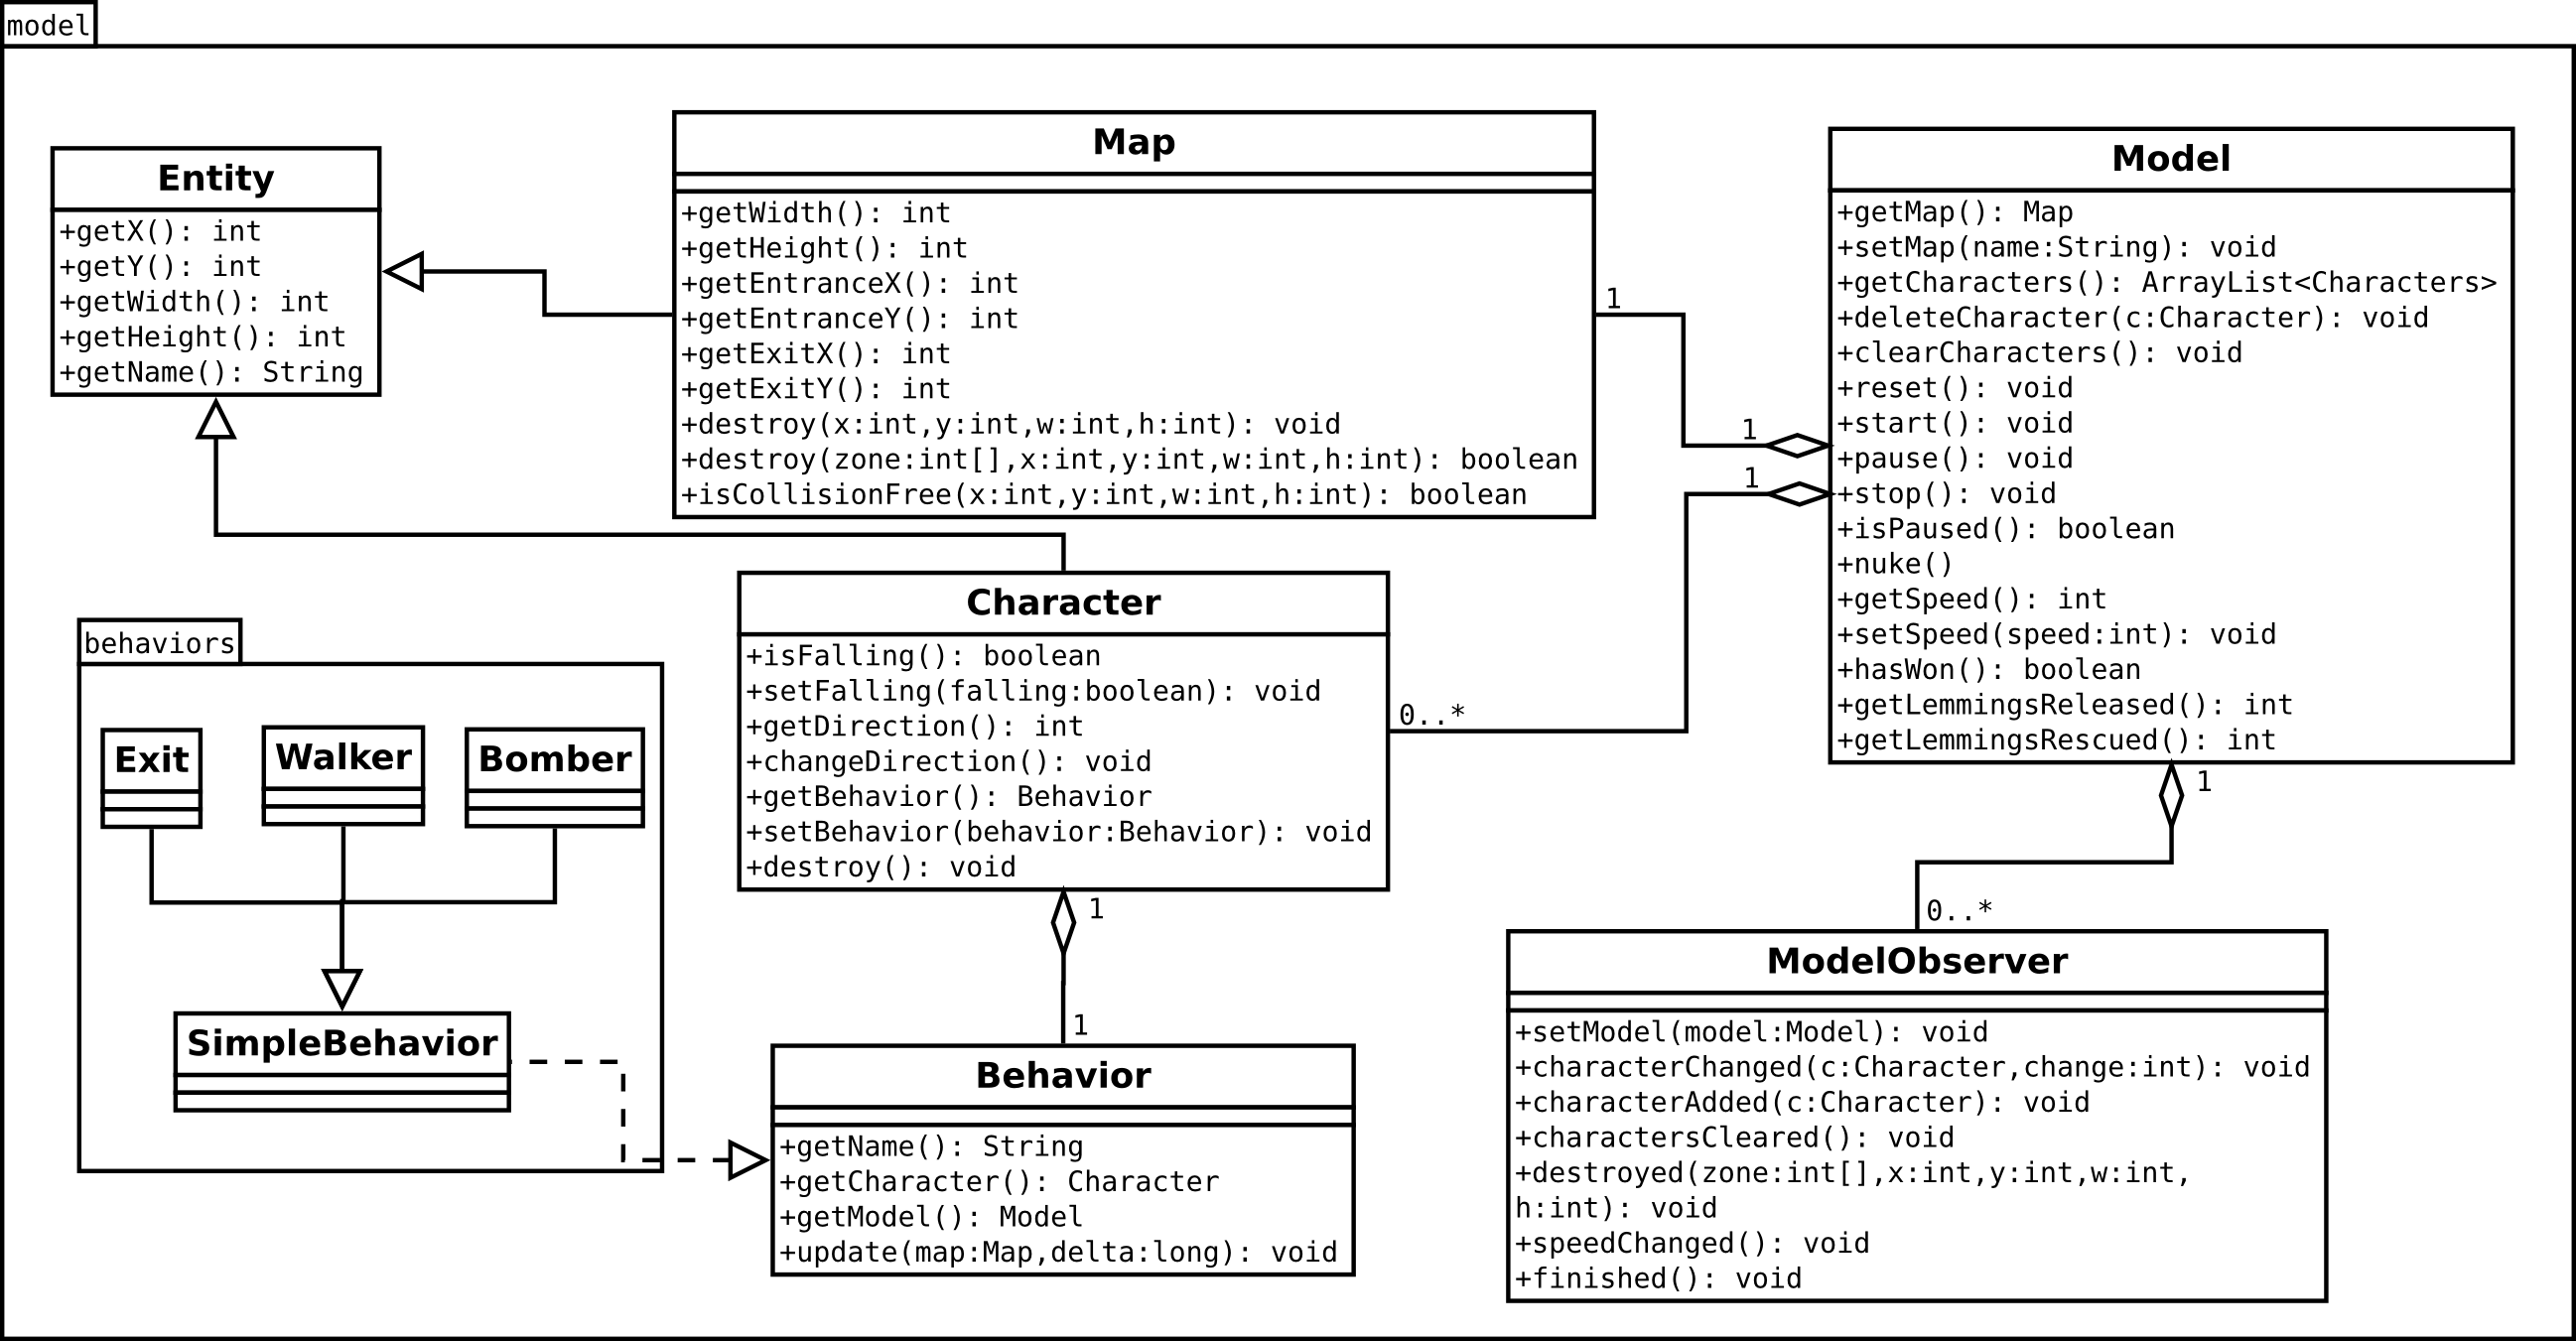
\includegraphics[width=\textwidth]{model.png}}
  \caption{Diagramme de classe du package \texttt{model}}
\end{figure}

La carte contient les données relatives aux collisions (un tableau
d'entier permettant de savoir si une position est accessible ou pas)
ainsi que la position de l'entrée et de la sortie. Une carte est
stockée sur le disque dur sous forme d'un dossier contenant les images
suivantes:
\begin{list}{-}{}
  \item \texttt{background.png}: l'image qui sera affichée par la vue
    en arrière plan~;
  \item \texttt{foreground.png}: l'image qui sera affichée par la vue
    en avant plan~;
  \item \texttt{collision.png}: une image contenant les informations
    relative aux collisions: les pixels transparents sont traversables
    par le joueur, tandis que les autres pixels sont des obstacles~;
  \item \texttt{objects.png}: une image contenant les différents
    objets contenu sur la map: l'entrée et la sortie.  Chaque objet
    est représenté par un pixel d'une certaine couleur dans cette
    image.
\end{list}

Le personnage sont associés à un \emph{comportement}
(\texttt{Behavior}), selon le patron de conception d'état.  Chaque
comportement possède une méthode update, dans laquelle il effectue les
actions du personnage.\\

La classe \texttt{Model} possède une liste d'observateurs (qui
implémentent l'interface \texttt{ModelObserver}, selon le patron de
conception \emph{observateur/observé}. Lorsqu'une modification à lieu
au sein du modèle, ses observateurs seront notifiés.

\subsection{Vue}
Le package \texttt{view} contient tout ce qui se rapporte à
l'interface graphique du jeu. Le système de menu utilise le patron de
conception d'état, déjà présent dans la librairie graphique utilisée:
la classe \texttt{LemmingsGame} représente la classe principale du jeu
et hérite de \texttt{StateBasedGame}, tandis que les différents états
du jeux héritent de \texttt{BasicGameState}. Les transitions entre les
différents états sont représentées dans le diagramme états-transitions
de la figure \ref{fig:Etats}.

\begin{figure}[ht!]
  \centerline{
  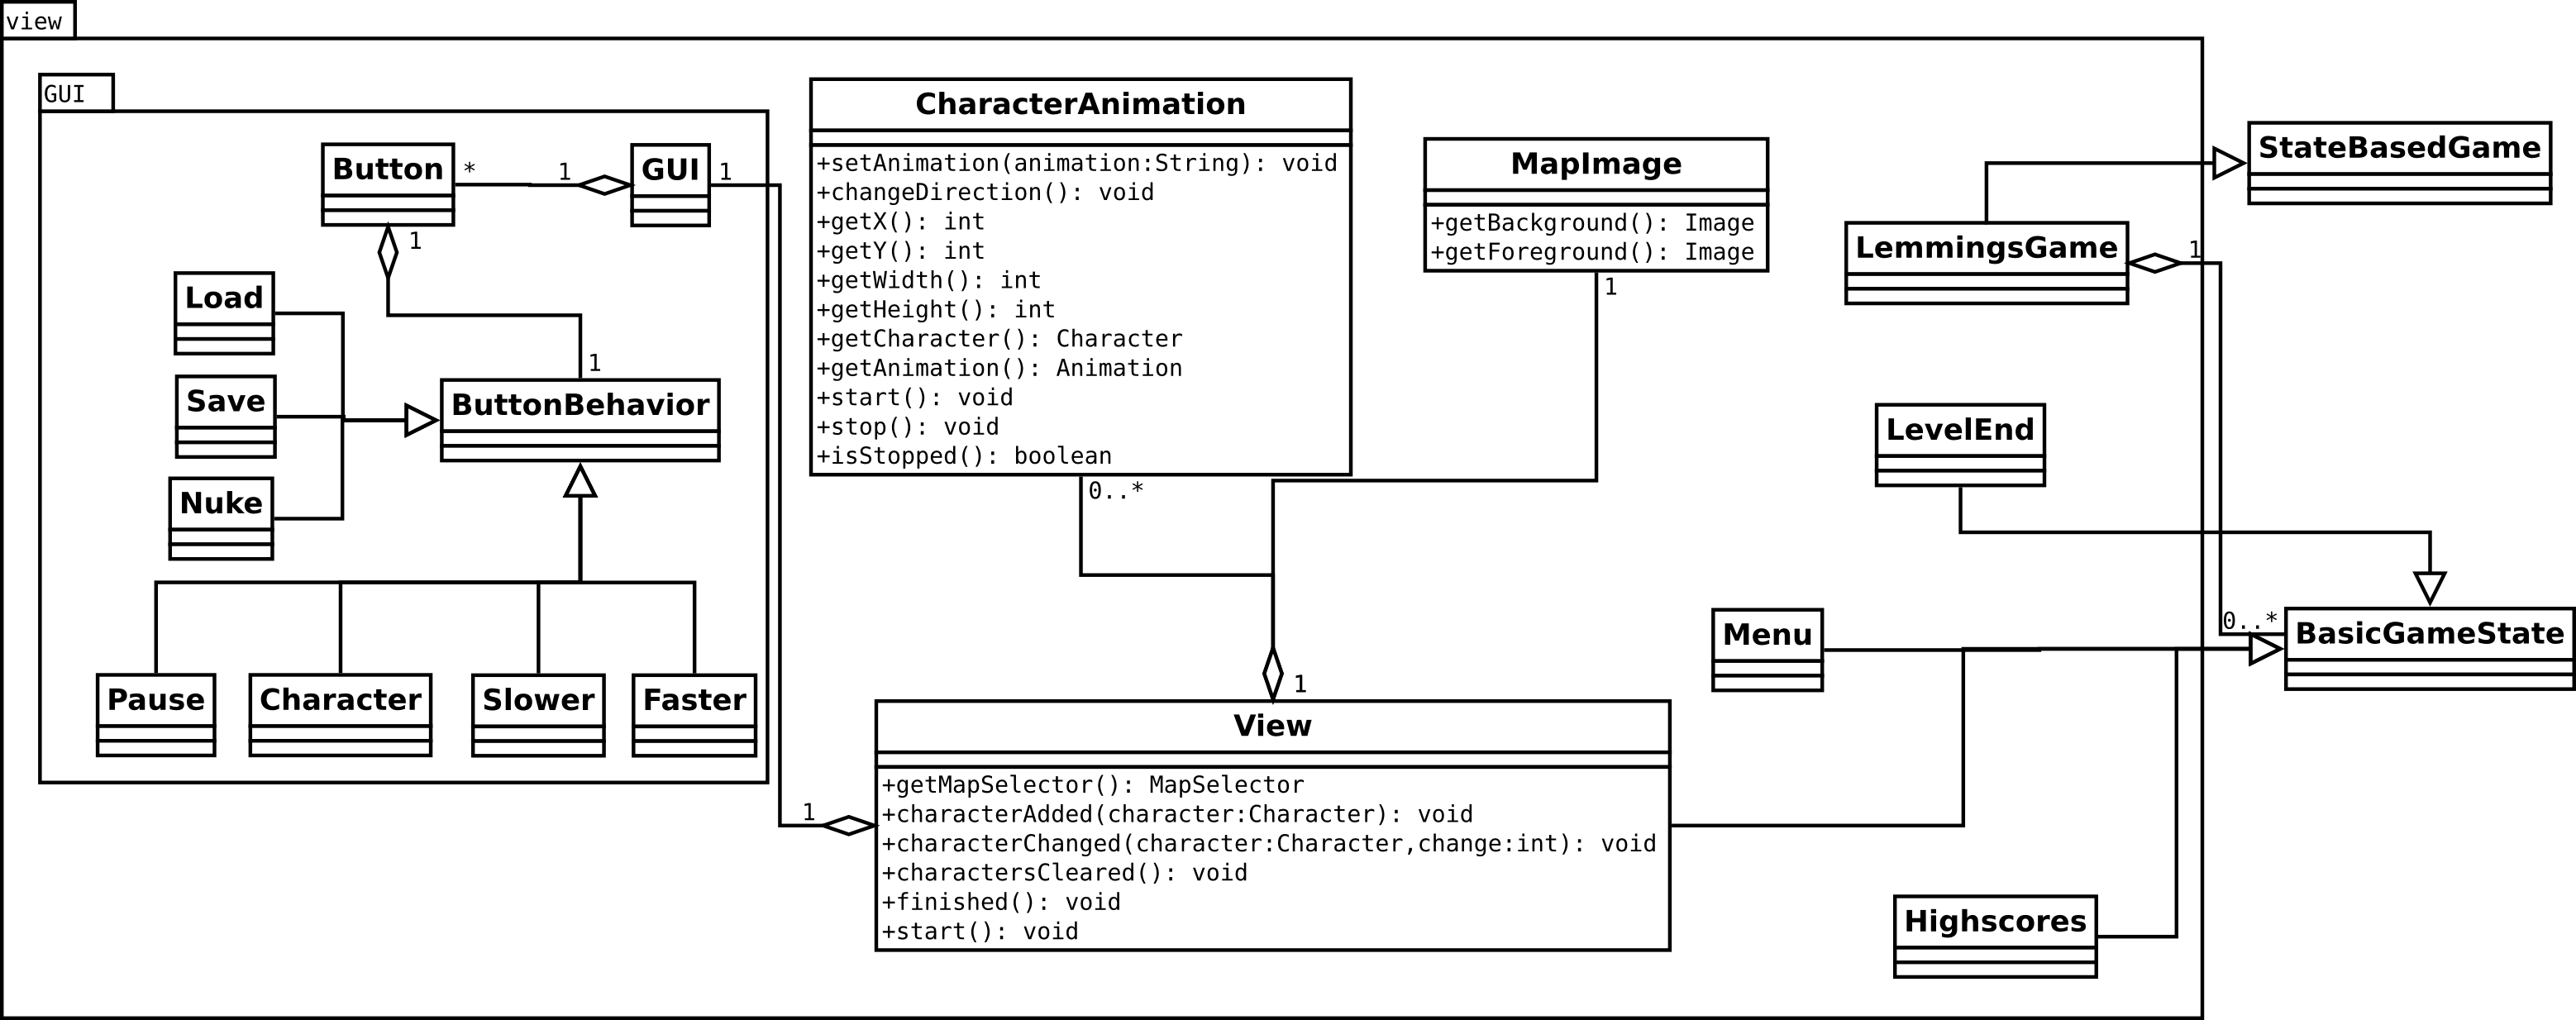
\includegraphics[width=\textwidth]{view.png}}
  \caption{Diagramme de classe du package \texttt{view}}
\end{figure}

\begin{figure}[ht!]
  \centerline{
  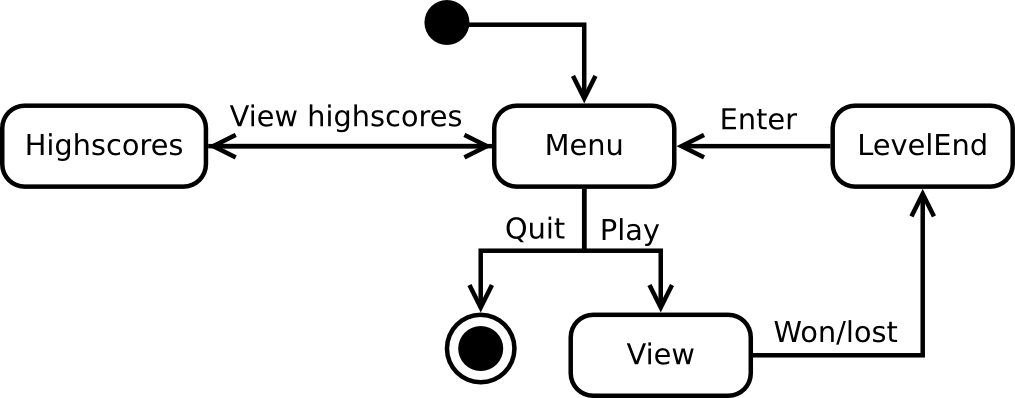
\includegraphics[width=0.6\textwidth]{state.png}}
  \caption{Diagramme états-transitions de l'interface graphique}
  \label{fig:Etats}
\end{figure}

L'état \texttt{View} est l'état principal du jeu: c'est cette classe
qui observe le modèle et l'affiche à l'écran. Elle contient un objet
de type \texttt{MapImage} qui représente les images de la carte
actuelle. Lorsque le terrain est creusé par un lemming, la vue en est
notifiée et la classe \texttt{MapImage} modifie la texture du terrain
pour tenir compte de ces modifications. La classe \texttt{View}
contient aussi une liste de \texttt{CharacterAnimation}, classe qui
permet d'afficher l'animation d'un personnage du modèle à l'écran.\\

Dernièrement, la classe \texttt{View} contient aussi un objet de type
\texttt{GUI}, qui implémente l'interface du jeu, composée de
différents boutons (classe \texttt{Button}) avec chacun un certain
comportement (\texttt{ButtonBehavior}). Lorsqu'un bouton est cliqué,
le controleur en est notifié et effectue les opérations nécessaires.\\

Les relations entre la vue et le modèle non représentées sur les
diagrammes de classes sont donc:
\begin{list}{-}{}
  \item la classe \texttt{CharacterAnimation} contient une référence
    vers le \texttt{Character} à laquelle elle correspond (relation
    un-à-un)~;
  \item la classe \texttt{View} implémente l'interface
    \texttt{ModelObserver}.
\end{list}

\subsection{Contrôleur}
Le contrôleur est implémenté dans l'unique classe
(\texttt{Controller}) du package \texttt{controller}. Cette
classe se contente de recevoir les événements de la vue
(bouton cliqué, personnage sélectionné, \dots) et d'appeler
les méthodes correspondantes du modèle.

\begin{figure}[ht!]
  \centerline{
  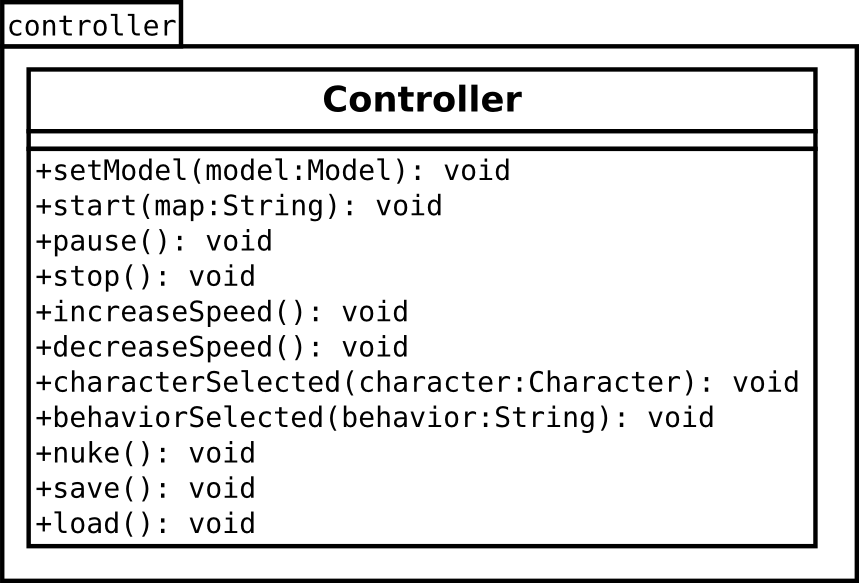
\includegraphics[width=0.55\textwidth]{controller.png}}
  \caption{Diagramme de classe du package \texttt{controller}}
\end{figure}

\subsection{Parser}
Les animations sont reprises du jeu \emph{Pingus}. Ces animations sont
stockées sous la forme de \emph{sprites} (une image contenant les
différentes étapes de cette animation). Le format de ces fichiers sont
décrits dans des fichiers \texttt{.sprite}, qui sont des fichiers avec
une syntaxe à base de \emph{s-expression}. La classe \texttt{LispFile}
permet de parser ces fichiers, qui sont représentés par un ensemble de
valeurs (classe \texttt{Value}). Cette classe est utilisée par la vue
pour charger les animations. Cela permet d'importer les images depuis
\emph{Pingus} sans devoir rajouter de code pour les charger dans le
programme.

\begin{figure}[ht!]
  \centerline{
  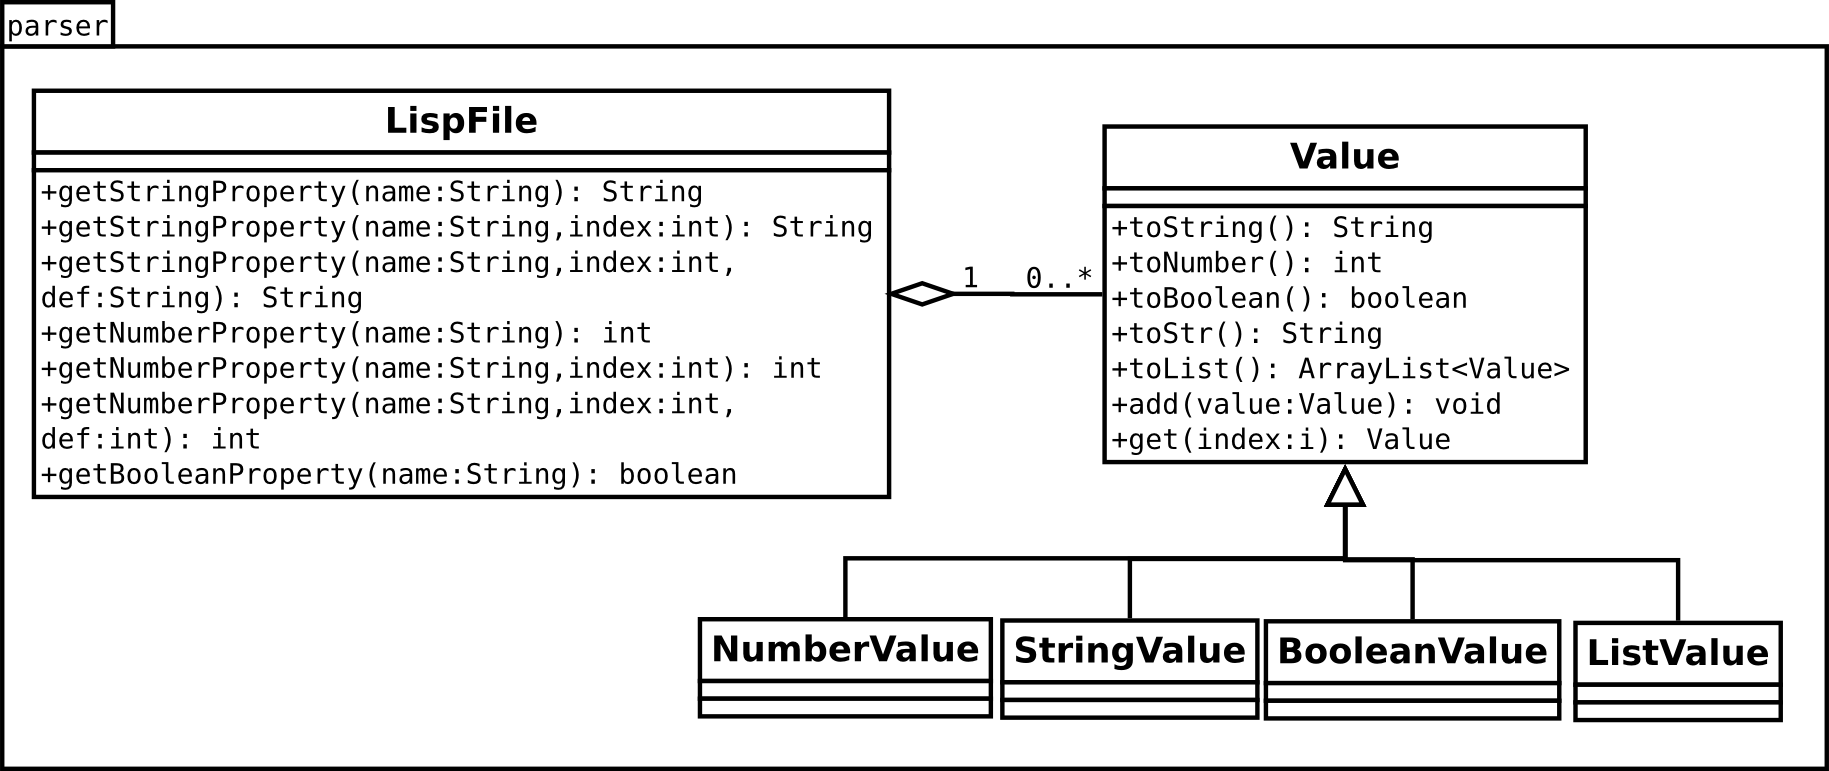
\includegraphics[width=\textwidth]{parser.png}}
  \caption{Diagramme de classe du package \texttt{parser}}
\end{figure}

\subsection{Outils}
Le package \texttt{util} contient quelques outils utilisés par le
reste du programme.\\

La classe \texttt{Selector} est une structure de donnée qui contient
un ensemble ordonné d'éléments, avec un pointeur vers un élément, qui
peut se déplacer vers la gauche ou vers la droite, d'une façon
similaire aux \texttt{ListIterator} de Java, mais en plus
convivial. Cette classe est utilisée par le menu pour permettre à
l'utilisateur de sélectionner la carte et la résolution.\\

La classe \texttt{LemmingsException} représente simplement une
exception qui s'est produite durant le jeu et est utilisée dans le
modèle et dans la vue.\\

La classe \texttt{Database} représente une connexion à la base de
donnée et permet de stocker les scores ainsi que différentes
options. Cette classe est implémentée selon le patron de conception
\emph{singleton}: toutes ses méthodes sont statiques, et lors du
premier appel à une de ses méthodes, la connexion à la base de donnée
est crée. Cette connexion est fermée dans le destructeur de cette
classe.\\

La classe \texttt{Score} représente une paire (nom, score) et est
utilisée par la classe \texttt{Database} pour retourner une liste de
score pour une certaine carte, afin d'être affiché dans la classe
\texttt{Highscore}.

\begin{figure}[ht!]
  \centerline{
  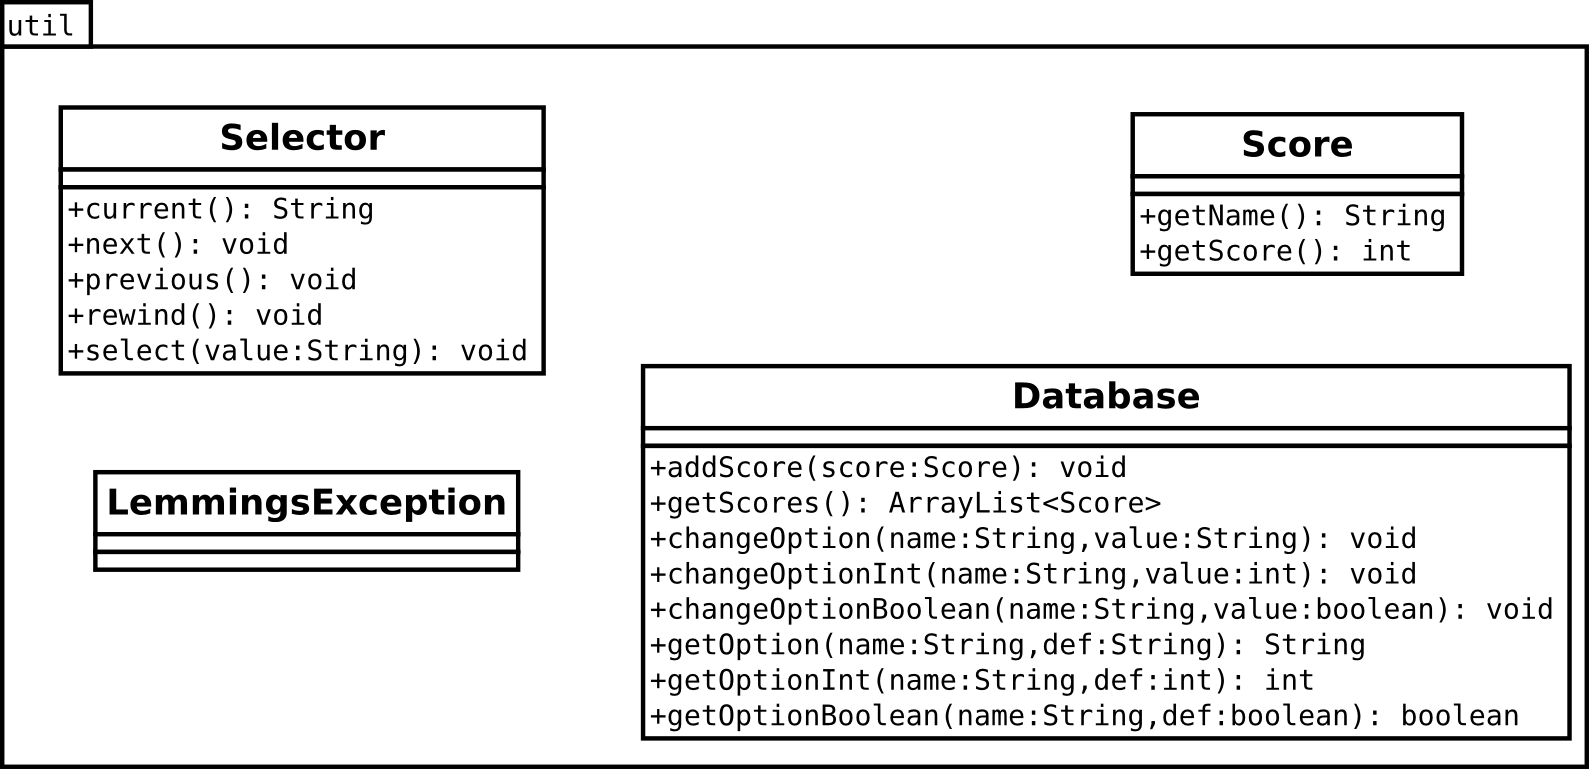
\includegraphics[width=\textwidth]{util.png}}
  \caption{Diagramme de classe du package \texttt{util}}
\end{figure}

\subsection{Relations entre packages}
Les relations entre les packages \texttt{model}, \texttt{view} et
\texttt{util} sont reprises dans le diagramme de classe à la figure
\ref{fig:Relations}.

\begin{figure}[ht!]
  \centerline{
  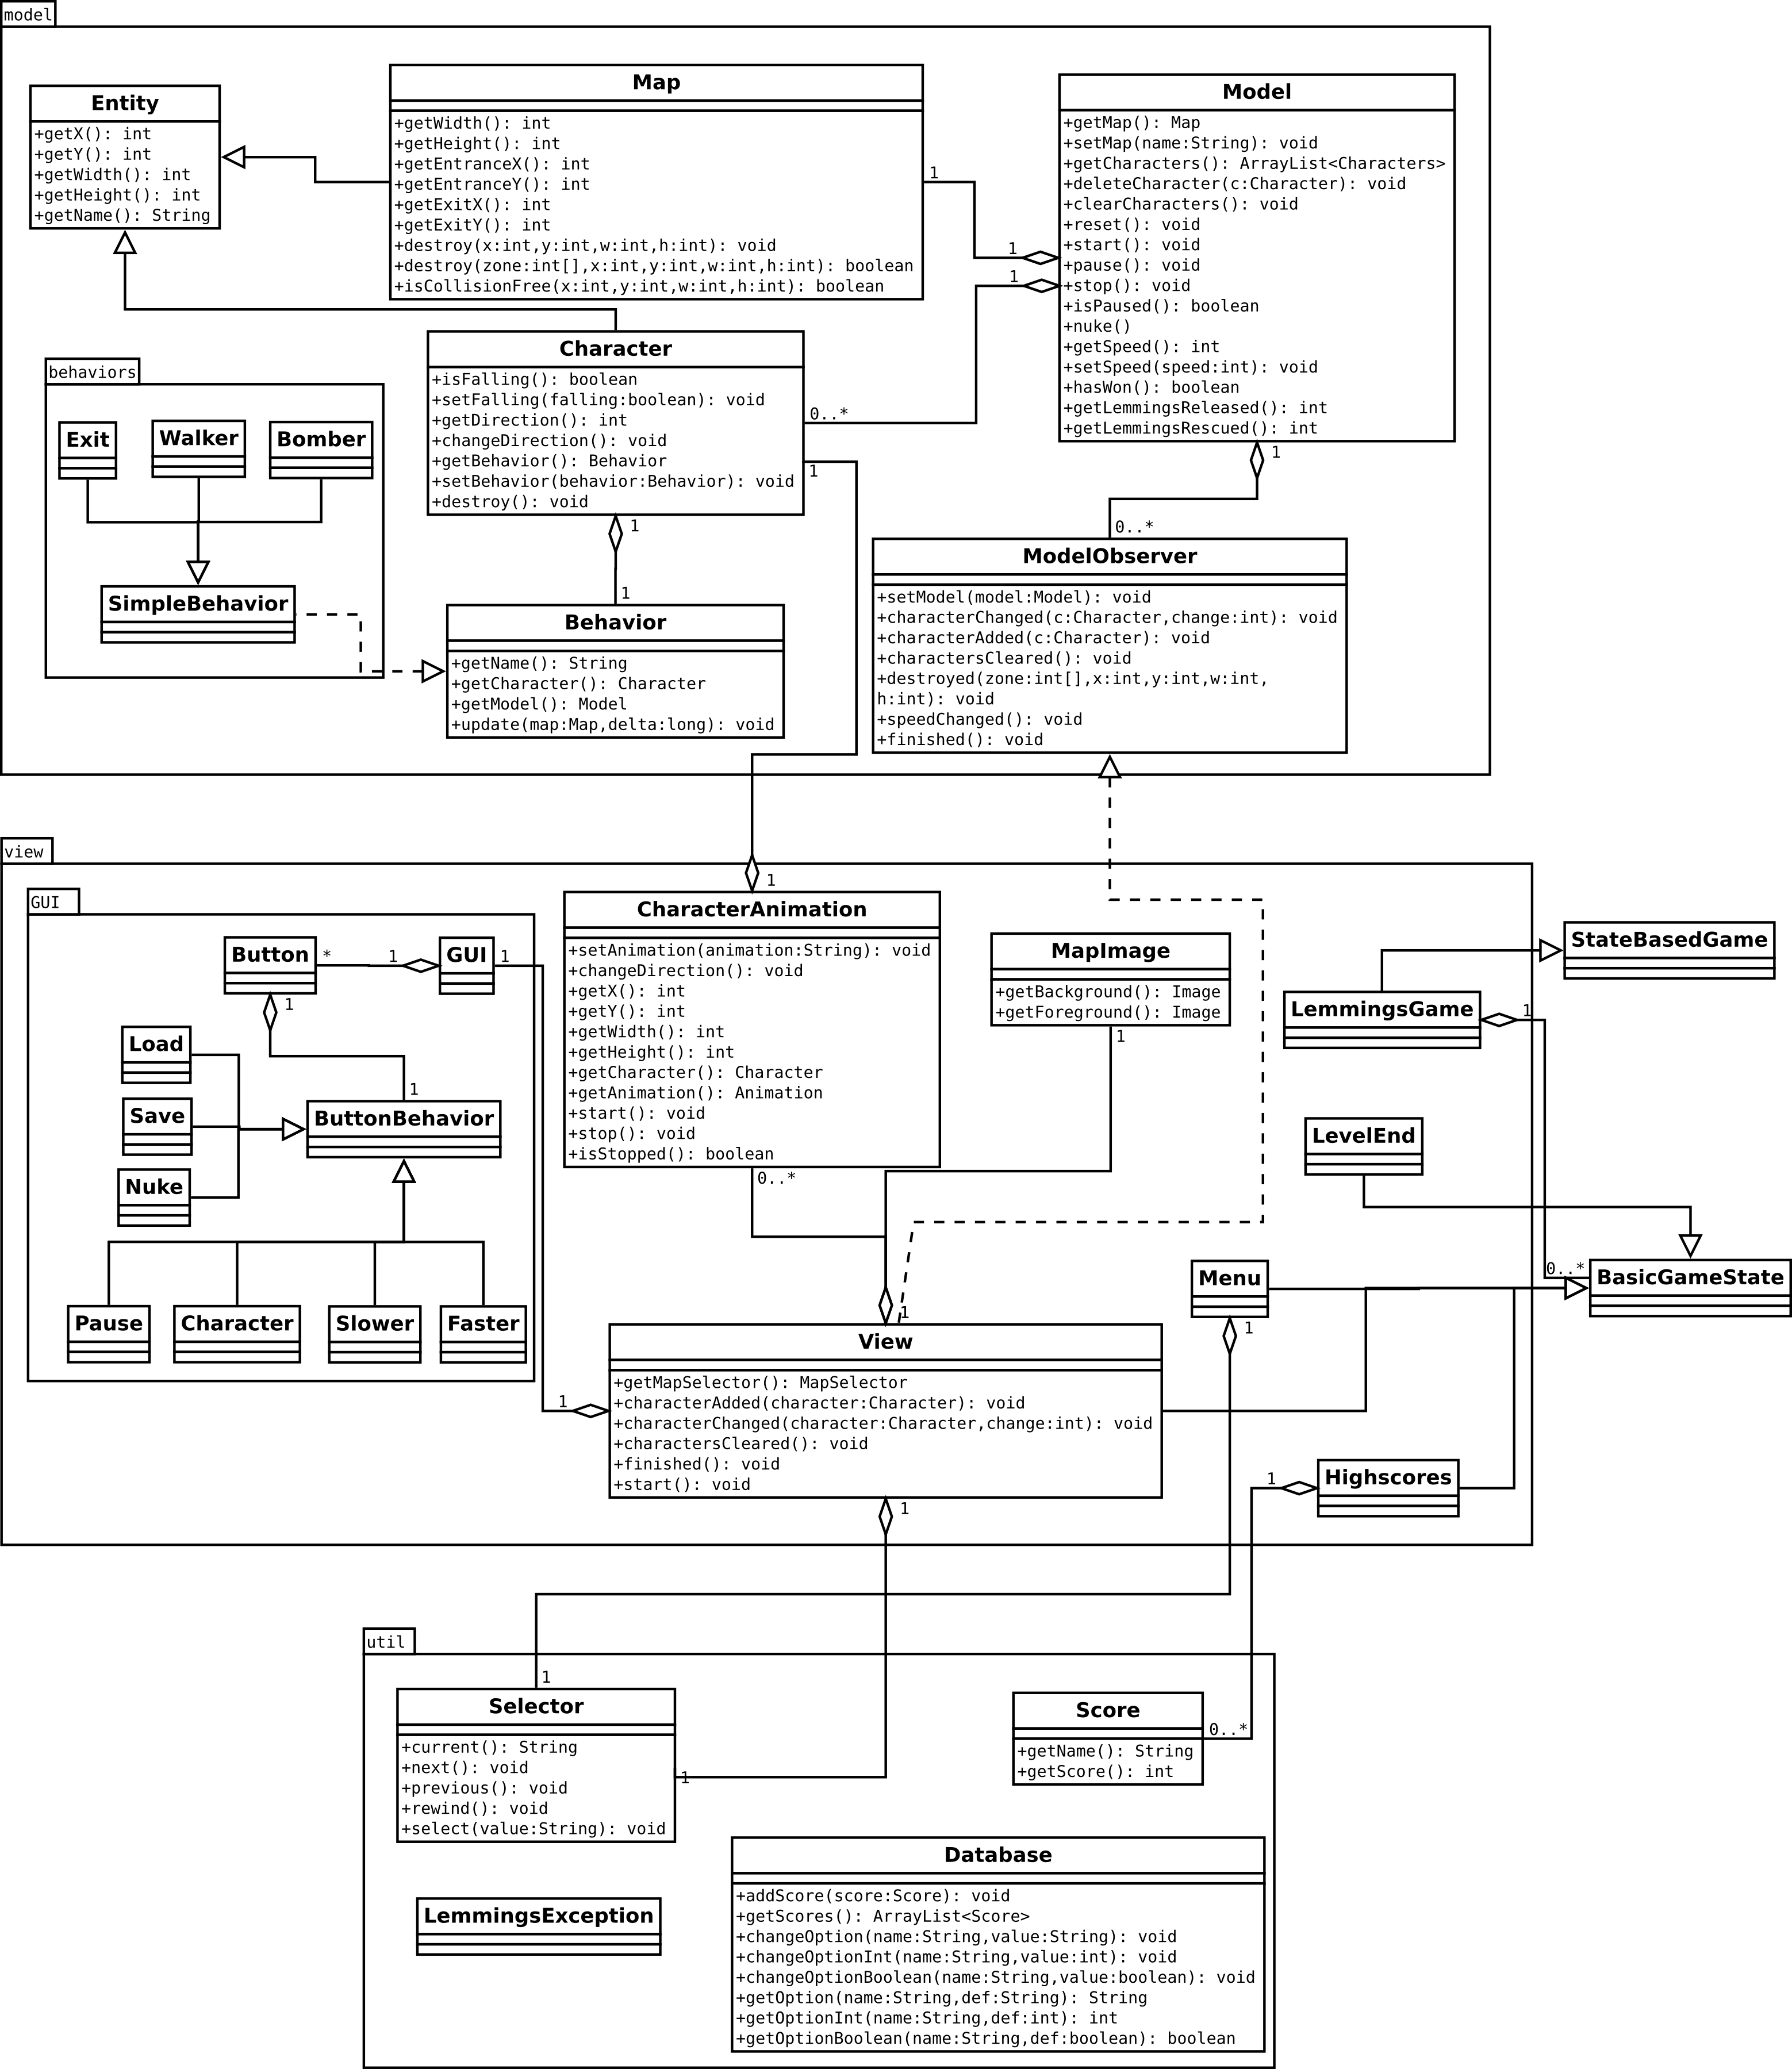
\includegraphics[width=0.9\textwidth]{relations.png}}
  \caption{Relations entre les différents packages}
  \label{fig:Relations}
\end{figure}

\end{document}
